% !Mode:: "TeX:UTF-8"

\chapter[非规范文本语义依存图分析]{非规范文本语义依存图分析}[Semantic Dependency Graph Parsing on Informal Texts]

\section{引言}[Introduction]
\label{sec:chapter3-intro}

神经网络在自然语言处理领域的应用,不仅解决了传统的基于特征工程的统计学习模型中对专家知识的依赖,更有效提升了该领域各个任务上模型的性能\cite{chen-manning-2014-fast,chiu-nichols-2016-named,ma-hovy-2016-end,zhou-etal-2016-text,chopra-etal-2016-abstractive}。
随着2018年BERT模型的提出,以其为代表的预训练模型为自然语言处理领域带来了新一波的显著性能提升\cite{peters-etal-2018-deep,devlin-etal-2018-bert,yang-etal-2019-xlnet,clark-etal-2020-electra}。
然而,尽管在自然语言处理领域中的很多数据集上,神经网络模型已经取得了接近甚至超过人类的效果,但近期的研究表明,现有的神经网络模型鲁棒性很弱。
与其在规范文本组成的数据集上取得的成功相对应的是其在非规范文本上性能的大幅下降\cite{alzantot-etal-2018-generating, ren-etal-2019-generating, cheng-etal-2019-robust,michel-etal-2019-evaluation, jin-etal-2020-isbert}。

对神经网络模型的鲁棒性进行研究的一般方式是对抗样本攻击(adversarial attack),即设计算法针对特定的目标模型(target model或victim model)生成使其产生误判的非规范文本。
这里的非规范文本并不是指有语法错误的文本,而是指与构建数据库常用的书面文本相对应的网络文本等不遵守严格书面文本规范的文本,其特点是包含有口语化的词汇,在语法上没有特别严格的要求。
而在对抗样本攻击中,这些被生成的文本一般被称为对抗样本(adversarial example)。
目前自然语言处理领域的鲁棒性研究工作一般选择情感分类、文本蕴涵等文本分类任务作为目标任务。
针对这些任务的特点,高质量的对抗样本需要满足两个条件:(1)在语义上与原始文本相同;(2)对原始文本的修改难以被察觉。
其中第一点的作用是保证在有标注数据上,修改后的对抗样本的类别不会因修改而改变,这样才能利用原始本文上的标注信息对攻击算法的性能进行评价。
而第二点从另一个角度来说,就是要保持对抗样本的流畅性,使得人类不会因文本的修改而对其类别产生误判。
因为使人类也产生误判的对抗样本对于模型的鲁棒性研究来说毫无作用,其可能就是完全无意义的词语组合。

尽管目前已有不少研究者针对上述以分类任务上神经网络模型的鲁棒性开展研究,但很少有人研究句法依存分析和语义依存图分析等结构化预测任务上的神经网络模型鲁棒性。
虽然这类任务无法直接应用到日常生活中,但其预测结果往往被用于帮助其他能直接应用的任务。
而一旦其性能因为非规范文本而显著下降,错误级联效应会导致使用其输出的其他任务模型性能也受到影响。

此前虽然有少量针对句法依存分析模型鲁棒性的研究工作,但其往往只注重攻击算法本身,而采用了简单的候选词生成方法,从而影响了生成的对抗样本的质量。
针对这一问题,本章首先设计了一套针对基于神经网络的依存分析模型的攻击算法,使用了多种候选词生成方法生成大量候选词,接着使用多种过滤方法将其中不合适的过滤掉,从而保证了候选词的质量和数量,最终实现了高质量对抗样本的生成。
接着,本章借助该对抗样本攻击算法对现存的多种依存分析模型和词向量的组合进行了攻击,并设计了多项实验研究基于神经网络的依存分析模型的鲁棒性。
最后,依据在分析实验中的发现,本章提出两种提升现有基于神经网络的依存分析模型鲁棒性的方法,分别是对抗样本训练(adversarial training)和模型融合。

为了验证上述对抗样本攻击算法的有效性,本章分别在中文语义依存图分析任务和英文句法分析任务上进行了实验,并组织了针对对抗样本质量的人工评价。
结果表明上述方法有效提升了生成的对抗样本的质量,而对抗样本训练和模型融合都能有效提高现有的基于神经网络的依存分析模型的鲁棒性。

\section{背景与相关工作}[Related Work]
\label{sec:chapter3-related-work}
与重视语义的分类任务不同,在依存分析等结构化预测任务上,高质量的对抗样本需要满足两个条件:(1)语义或句法结构与原始文本相同;(2)文本流畅性。
其中第二点与分类任务中的条件相同,也是为了保证对抗样本不使人类产生误判。
而第一点则是为了保证原始文本上的人工标注信息在对抗样本上依然有效,这与分类任务中第一个条件有类似之处,但对于结构化预测任务更为严格。
这是因为首先结构化预测任务上的标注信息不仅只有一个标签,而是一个复杂的结构。
其次,相比于分类任务,结构化预测任务的标注更难以获取。
要使用正确的标注信息对攻击算法进行评价,往往只能保证修改后的文本上的结构不变。
正如第\ref{sec:chapter3-intro}节所介绍,目前虽然有少量针对句法依存分析模型鲁棒性的研究工作,但其往往忽略了对抗样本的质量。
本节将重点介绍与本章研究内容密切相关的针对依存分析模型鲁棒性进行研究的工作。

Zheng等人\cite{zheng-etal-2020-evaluating}于2020年在英文上首次开展了针对基于神经网络的句法依存分析模型的鲁棒性研究。
他们使用BERT模型基于上下文预测每个词的候选词,然后选择使目标模型性能下降最大的候选词替换原始文本中的词,从而实现对句法依存分析器的攻击。
具体来说,本文第\ref{sec:chapter1-informal}节已经介绍了BERT使用的遮盖语言模型训练目标,即通过将目标词遮盖然后用其上下文预测该词。
而该方法依次将目标句子中的每个词用BERT模型中特殊的遮盖符号进行替换,然后用BERT模型对该词进行预测,从而获取BERT模型词表中所有词在文本中该位置出现的概率。
然后再对这些词按照出现概率进行排序,选取其中前$N$个作为候选词。
需要特别说明的是,由于英文BERT模型使用的是词片段(word piece)向量而非词向量,其词表中很多都是不完整的词片段而非整词。
而不完整的词片段显然是无法替代原始句子中完整的词的,因此该方法只选择出现概率高的候选词中的整词作为候选词。
显然这种方法严重限制了候选词的多样性,而且由于英文中大部分复杂的词在BERT中都会被切割成词片段,这种方法无法生成这些复杂的词。

Han等人\cite{han-etal-2020-adversarial}于2020年在英文上开展了针对结构化预测任务上的神经网络模型的鲁棒性研究,并在句法依存分析任务上进行了实验。
他们提出一个序列到序列(sequence-to-sequence)模型,根据输入的原始文本生成对抗样本。
由于该模型无法保证生成的对抗样本与原始文本长度相同或具有相同的结构,该方法使用了两个额外的依存分析器的预测结果作为参考。
这两个额外的依存分析器与目标依存分析器要求是两两不同的依存分析模型,这样才能保证其预测结果与受攻击的目标分析器不同,且两个参考依存分析器之间才能互相验证。
该方法对于目标分析器和参考分析器的类别有较严格的要求,而且尽管其通过限制分析器类别提升了作为参考的预测结果的准确性,该方法仍然无法保证预测结果是完全正确的。
在这种情况下,使用预测的结果作为对抗样本正确标注对攻击方法进行评估也难以保证其准确率。

总的来说,此前的针对基于神经网络的依存分析模型的鲁棒性研究集中在英文的句法依存分析任务上,且往往忽略了生成的对抗样本质量。
而在对抗样本攻击中,对抗样本的质量是十分重要的,低质量的对抗样本很可能使人类也产生误判,从而对于模型鲁棒性的研究没有贡献。
另外,在对模型鲁棒性研究的基础上,如何提升依存分析模型的鲁棒性,也是亟待解决的问题。
因此,本章首先设计了针对依存分析模型生成高质量对抗样本的攻击算法,然后利用该算法对现有的依存分析模型鲁棒性进行研究,并在此基础上提出了提升其鲁棒性的方法。

\section{针对依存分析器的对抗样本攻击算法}[Adversarial Attacking Framework against Dependency Parsers]

正如本文第\ref{sec:chapter1-informal}中所介绍的,根据攻击者对被攻击模型的了解程度,对抗样本攻击可以分为白盒攻击和黑盒攻击两类。
在白盒攻击情境下,攻击者能获取目标系统的所有信息,包括模型结构,参数及权重值等。
而在黑盒攻击情境下,攻击者仅能用对目标系统查询的方式,通过输入观察输出结果。
显然在现实应用场景中,白盒攻击的条件是很难达成的。
因此本章选择更贴近现实应用场景的黑盒攻击情境,设计了一个针对依存分析模型的黑盒攻击算法,生成高质量的对抗样本。

%研究表明,在深度神经网络输入中加入微小扰动信息,能够使其产生误判。
%这种使神经网络产生误判的攻击称为对抗样本攻击,其中使用的输入样本称为对抗样本。
%尽管基于深度神经网络的模型在自然语言处理领域的很多任务上都取得了很好的成果,但对抗样本攻击揭示了这类模型脆弱的一面。
%为了提高现有依存分析器的鲁棒性,使其适用于现实复杂场景,我们首先设计对抗样本攻击算法,针对现有各类依存分析器生成对抗样本,并对生成的样本进行分析,在此基础上提出了增强分析器鲁棒性的方法。

下面首先给出针对依存分析模型进行对抗样本攻击的形式化定义。
给定包括所有可能输入句子$\bm{x}$的输入文本空间$\mathcal{X}$和包括$\bm{x}$所有可能依存结构的输出空间$\mathcal{Y}$。
一个依存分析模型$F: \mathcal{X} \rightarrow \mathcal{Y}$的目标是学习一个从输入句子$\bm{x}$到其对应依存结构$\bm{y}$的映射,记为$F(\bm{x}) = \bm{y}$。
句子$\bm{x}$中的第$i$个词记为$x_i$,用$(i,j,r) \in \bm{y}$表示依存结构$\bm{y}$中存在一条由$x_i$指向$x_j$,标签为$r$的弧。

给定一个句子$\bm{x}$,本章通过对其进行微小的修改获得$\bm{x}^*$,当$\bm{x}^*$满足以下条件时,将其称为一个有效的对抗样本:
$$F(\bm{x}^*) \neq \bm{y}, \sigma(\bm{x}^*, \bm{x})\le \epsilon, $$
其中$\sigma$为样本变化约束函数,$\epsilon$则限制了生成的对抗样本$\bm{x}^*$需要满足两个条件:(1)对抗样本相对于原始文本的变化足够小;(2)对抗样本的正确依存结构与原始文本的正确依存结构相同。
这两个条件是第\ref{sec:chapter3-related-work}中提出的结构化预测任务上高质量对抗样本需要满足的条件在对抗样本攻击中的具体体现。
在本章提出的方法中,通过使用多种候选词生成方法和多种候选词过滤方法来确保他们。
在实验中,本章将分别采用流畅性和依存结构不变性两个评价指标对生成的对抗样本是否满足这两个条件进行评价。

本章提出的针对依存分析模型的黑盒攻击算法如算法\ref{algo:attack}所示,由词重要性排序(1-4行)、候选词生成(第7行)和替换词搜索(8-28行)三部分组成。
其核心思想是对句中每个词生成若干能保证流畅性和依存结构不变性的候选词,按照句中词的重要性由高到低搜索并替换能使目标分析模型预测准确率下降的候选词。
接下来对这三个部分进行具体介绍。

\begin{algorithm}[!h]
    \wuhao
	%\begin{flushleft}
	%	\textbf{Input:} 原始样本 $\bm{x}^{(0)}=\{x_1,x_2,\dots,x_N\}$, 最大允许修改百分比 $\gamma$ \\
	%	\textbf{Output:} 对抗样本 $\bm{x}^{(i)}$
	%\end{flushleft}
	\LinesNumbered %要求显示行号
    \KwIn{原始样本 $\bm{x}^{(0)}=\{x_1,x_2,\dots,x_N\}$, 最大允许修改百分比 $\gamma$}%输入参数
    \KwOut{对抗样本 $\bm{x}^{(i)}$}%输出
		\For{$i=1$ to $N$}
		{
		    用公式\ref{eq:word-importance}计算词重要性$I(\bm{x}^{(0)},x_i)$\;
		}
		建立一个由$x_i\in\bm{x}^{(0)}$组成的集合$W$,其中词按照重要性$I(\bm{x}^{(0)},x_i)$从高到低排序\;
		$t=0$\;
		\For{$W$中每个$x_j$}
		{
		    按照候选词生成步骤建立词$x_j$的候选词集合$\mathcal{C}_j$\;
		    初始化有效候选词集合$\mathcal{VC} \leftarrow \{\}$\;
		    \For{$\mathcal{C}_j$中每个候选词$c_k$}
		    {
		        用公式\ref{eq:mis-inc}计算准确率改变量$S(\bm{x}^{(t)},c_k,j)$\;
		        \If{$S(\bm{x}^{(t)},c_k,j) > 0$}
		        {
		            将$c_k$加入集合$\mathcal{VC}$
		        }
		        %\algorithmicif\  $S(\bm{x}^{(t)},c_k,j) \le 0$\ \algorithmicthen\ continue\ \algorithmicendif\
		        %将$c_k$加入集合$\mathcal{VC}$\;
		    }
		}
		\If{$\mathcal{VC}$非空}
		{
		    $c^* = \argmaxl_{c \in \mathcal{VC}} S(\bm{x}^{(t)},c,j)$\;
    		$t = t + 1$\;
    		$\bm{x}^{(t)} \leftarrow \text{将} \bm{x}^{(t-1)} \text{中的} x_j  \text{替换为} c^*$\;
    		\If{$t \ge \gamma \cdot N $}
    		{
    		    \algorithmicreturn\ $\bm{x}^{(t)}$
    		}
    		%\algorithmicif\  $t \ge \gamma \cdot N $\ \algorithmicthen\   \algorithmicreturn\ $\bm{x}^{(t)}$\ \algorithmicendif\;
		}
		\eIf{$t > 0$}
		{
		    \algorithmicreturn\ $\bm{x}^{(t)}$
		}
		{
		    \algorithmicreturn\ None
		}
		%\algorithmicif\  $t > 0$\ \algorithmicthen \algorithmicreturn\ $\bm{x}^{(t)}$\ \algorithmicelse\ \algorithmicreturn\ None \algorithmicendif
	\AlgoBiCaption{针对依存分析器的黑盒攻击算法}{Black-box attack algorithm against dependency parsers.}
	\label{algo:attack}
	%\bicaption[algo:attack]{算法}{针对依存分析器的黑盒攻击算法}{Algo.$\!$}{Effect of different modules of BS-IT model.}
\end{algorithm}


\subsection{词重要性排序}[Word Importance Ranking]

在一个句子中,不同的词对于模型的预测结果会产生不同程度的影响,本章将这种影响的大小视为词的重要性,对句中词按重要性进行排序。
此前的方法通过将句中词逐个替换为未知标签并计算替换前后模型预测结果的改变获得词的重要性。\cite{li-etal-2016-visualizing,ren-etal-2019-generating}
针对依存分析任务,本章使用依存分析性能的改变量作为衡量词重要性的分数。
具体来说,对于英文句法分析本章使用无标记依存正确率(Unlabled Attachment Score,简称UAS)和带标记依存正确率(Labled Attachment Score,简称LAS)。
对于中文语义依存图分析本章使用不计算弧标签的F值(UF)和计算弧标签的F值(LF)。
这二者的区别是由于句法依存树中每个词只有一个父节点,因此可以直接将准确率作为评价指标,而语义依存图中每个词的父节点数量不确定,因此需要用F值作为评价指标。
在下文的攻击方法描述中,统一使用句法分析评价指标为例,当攻击目标为语义依存图分析时,只需要将UAS替换为UF、LAS替换为LF。
具体来说,句子$\bm{x}$中词$x_i$的重要性为:
\begin{equation}
	\label{eq:word-importance}
	I(\bm{x},x_i) = \lambda_{\text{arc}}\Delta_\text{UAS}(\bm{x},\hat{\bm{x}_i}) + (1-\lambda_{\text{arc}})\Delta_\text{LAS}(\bm{x},\hat{\bm{x}_i}),
\end{equation}
其中$\bm{x} = x_1x_2\dots x_i\dots x_N$为原始句子,$\hat{\bm{x}_i} = x_1x_2\dots \text{UNK}\dots x_N$为将词$x_i$替换为特殊未知词标签UNK的修改后句子。
$\Delta_\text{UAS}(\bm{x},\hat{\bm{x}_i}) = \text{UAS}(F(\bm{x})) - \text{UAS}(F(\hat{\bm{x}_i})) $和$\Delta_\text{LAS}(\bm{x},\hat{\bm{x}_i}) = \text{LAS}(F(\bm{x})) - \text{LAS}(F(\hat{\bm{x}_i}))$分别表示修改前后UAS和LAS的改变量。
$\lambda_{\text{arc}}$为用于调节依存弧和标签之间相对重要性的系数。


\subsection{候选词生成}[Generation of Substitute Candidates]
\label{sec:gen-cand}

候选词生成是本章提出的攻击算法中重要的一步,生成的候选词的数量和质量决定了攻击时的搜索空间和对抗样本的质量。
本文第\ref{sec:chapter3-related-work}节中介绍了此前工作使用的基于预训练语言模型BERT生成候选词的方法,受到BERT本身词片段表示形式的制约,这种方法生成的候选词也受到了严重限制。
此外,与使用词片段向量作为输入的英文BERT不同,现存的中文BERT使用字向量作为输入,这种情况也使该方法无法直接应用到中文语义依存图分析模型的攻击中。
为了同时保证生成的候选词的数量和质量,本章首先使用四种候选词生成方法生成大量候选词,然后使用三种过滤方法过滤掉其中不合适的候选词。
%此前的工作尝试了包括基于语言模型的\cite{zheng2020evaluating}、基于词向量的\cite{alzantot2018generating}、基于同义词的\cite{ren2019generating}和基于义原(Sememe)的\cite{zang2020word}生成方法。
%这些方法各自存在不同的问题,前两类生成的候选词质量无法保证,而后两类生成候选词的数量受到限制。
%为了解决这些问题,我们首先同时用这四类方法生成候选词集合,之后使用四种过滤方法过滤掉不合适的候选词,从而同时保证了候选词的质量和数量。

接下来首先具体介绍本章使用的四种候选词生成方法:

1.\textbf{基于BERT的方法}\cite{zheng-etal-2020-evaluating}。
本章提出的攻击算法能够同时攻击中文和英文依存分析模型。
由于目前中英文的BERT采用了不同类别的输入向量,这里将分别介绍中英文的情况。

针对英文,本章采取与第\ref{sec:chapter3-related-work}节中介绍的Zheng等人相同的方法,将原始句子中的词逐个遮盖,然后使用英文BERT基于其上下文预测词表中所有词出现在此上下文中的概率。
之后对这些词按照出现概率排序,选择前$k$个整词(没有被切分成片段的词)作为当前词的候选词。

针对中文,由于中文BERT采用字向量而非词片段向量作为输入,本章采用分别计算组成一个词的各个字在上下文中的出现概率,然后用多个字同时概率作为候选词概率的方式来生成候选词。
具体来说,假设当前目标词$x=d_1d_2\dots d_N$由$N$个字组成。
本方法逐个将其中的每个字遮盖,利用中文BERT基于上下文预测每个可能的字出现在此处的概率。
将字$s_i$出现在$i$位置,替换字$d_i$的概率记为$p(d_i\rightarrow s_i)$。
则候选替换词$x'=s_1s_2\dots s_N$的概率为$p(x\rightarrow x') = \prod_{i=0}^{N}p(d_i\rightarrow s_i)$。
然而由于本方法在每个位置预测的都是所有可能出现的字,全排列组合中的有些词可能是没有意义的。
为了避免将这种没有意义的词也作为候选词,本方法会对组合后的词使用中文词表进行过滤,只保留在中文词表中的有意义的词。
过滤后,对剩余的词按照$p(x\rightarrow x')$进行排序,选取其中前$k$个作为当前词的候选词。

2.\textbf{基于词向量的方法}\cite{alzantot-etal-2018-generating}。
该方法使用预训练的固定词向量,计算各词之间的词向量余弦相似度,目标词的$k$个最近的词作为其候选词。
需要注意的是,在一般的词向量中,距离近的词不仅有近义词,也有反义词。
这是因为一般的词向量训练方法只是根据词在上下文中的出现情况学习其向量表示,而同义词和反义词都容易出现在相同的上下文中。
为了解决这一问题,本章使用Mrksic等人\cite{mrksic-etal-2016-counter}提出的方法对预训练固定词向量进行预处理。
具体来说,该方法在预训练词向量中加入了来自近义词和反义词词典的约束,在保证词向量之间相对位置不变的同时缩短近义词向量间的距离,扩大反义词向量建的距离。
这种预处理使该方法生成的候选词更有可能是近义词,从而提高了其质量。
对于英文,该方法使用预处理过的GloVe词向量\cite{pennington-etal-2014-glove}计算余弦相似度。
对于中文,该方法首先Word2vec方法\cite{mikolov-etal-2013-distributed}在中文Gigawords语料\footnote{\url{https://catalog.ldc.upenn.edu/LDC2011T13}}上训练固定词向量,然后用上述方法对其进行预处理,最后计算余弦相似度。

3.\textbf{基于近义词的方法}\cite{ren-etal-2019-generating}。
该方法从近义词词典中获取目标词的近义词作为候选词。
对于英文,该方法使用WordNet\footnote{\url{https://wordnet.princeton.edu}}获取目标词的近义词。
对于中文,该方法使用哈工大同义词词林获取目标词的近义词。

4.\textbf{基于义原的方法}\cite{zang-etal-2020-word}。
Dong等人\cite{dong-etal-2006-hownet}于2006年提出了基于义原的语言知识库——知网(HowNet)。
义原在语言学中指最小的不可再分的语义单位, 对于每个候选词,该方法根据知网中定义的义原,收集词表中所有至少有一个义原与其重复的词作为其候选词。
例如,假设目标词为“中文”,其在知网中的的义原包括“中国”和“语言”,对于词表中的词“英文”,其在知网中的义原包括“英国”和“语言”。
由于“英文”的义原与“中文”的义原中都包含“语言”,该方法将“英文”作为“中文”的候选词。
知网中定义的义原包括中文和英文两部分,因此针对中英文方法都统一使用知网中定义的义原来获取其候选词。

在用上述方法获得大量候选词之后,本章依次使用以下三种过滤方法,将所有候选词中不合适的过滤掉:

1.\textbf{词性过滤方法}。
该方法过滤掉候选词中与目标词词性不同的,这是为了确保替换后依存结构不变。
具体来说,对于原始句子$\bm{x} = x_1x_2\dots x_i\dots x_N$,假设当前目标词为$x_i$,则依次用每一个候选词$x'_i$替换$x_i$,然后使用斯坦福词性标注器对新的序列$x_1x_2\dots x'_i\dots x_N$进行词性标注。
如果获得的$x'_i$的词性与$x_i$的原始词性(从依存语料库中获取)不同,则将候选词$x'_i$过滤掉。

%\textbf{语法检测过滤} \ \ 我们使用公开的语法检测工具\footnote{\url{https://pypi.org/project/language_tool}}过滤掉替换后会引入语法错误的候选词,从而进一步确保句法结构的不变性和语法的正确性。

2.\textbf{词向量相似度过滤方法}。
该方法计算当前目标词与其每个候选词的词向量余弦相似度,然后过滤掉其中相似度低于$\epsilon_w$的候选词。
其目的是为了通过尽可能提高目标词与候选词的相似性来提高生成的对抗样本的流畅性。
因此这里使用的是基于词向量的生成方法中经过预处理的预训练固定词向量。

3.\textbf{困惑度过滤方法}。
为了进一步提高生成的对抗样本的流畅性,该方法使用替换后句子的困惑度(perplexity)增量对候选词进行过滤。
具体来说,对于原始句子$\bm{x}$中第$i$个词$x_i$的每个候选词$c$,该方法使用预训练的语言模型计算原始句子$\bm{x}$和替换后句子$\bm{x}^c_{i}$的困惑度,定义困惑度增量为:
\begin{equation}
	\label{eq:ppl-inc}
	\Delta \text{ppl}(\bm{x},c,i)= \text{ppl}(\bm{x}^c_{i})-\text{ppl}(\bm{x}),
\end{equation}
其中$\bm{x}^c_{i}$为将原始文本$\bm{x}$的第$i$个词替换为$c$后的文本,$\text{ppl}(\bm{x})$表示使用预训练模型计算的序列$\bm{x}$的困惑度。
使$\Delta\text{ppl}(\bm{x},c,i) > \epsilon_p$的候选词将被过滤掉。

困惑度是用来评价语言模型的指标,对于输入句子$\bm{x} = x_1x_2\dots x_i\dots x_N$,其困惑度为:
\begin{equation}
    \text{ppl}(\bm{x}) = p(w_1w_2\dots w_N)^{-\frac{1}{N}}
\end{equation}
其中$p(w_1w_2\dots w_N)$表示使用语言模型计算的该句子出现的概率。
在固定的由正常句子组成的测试集上,困惑度越小,代表这些正常的句子出现的概率越大,也就说明语言模型越好。
而当使用一个固定的预训练好的语言模型时,对于给定的句子,困惑度越小说明其出现概率越大,也即这个句子是正常句子的概率越大。
从另一个角度也就是说这个句子的流畅性越高。
通过限制候选词带来的困惑度提升,该方法能有效提高生成对抗样本的流畅性。
该方法分别选用中文和英文的预训练语言模型GPT-2\cite{radford-etal-2019-language}来计算句子困惑度。

\subsection{替换词搜索}[Best Substitute Searching]

在第一步获取的词替换顺序和第二步获取的高质量候选词的基础上,本章用贪心搜索策略搜索合适的候选词替换原始句子中的词。
在对抗样本攻击时,不允许替换代词、冠词、连词、数字、感叹词、限定疑问词和标点符号。
这是因为这些词的替换不仅容易改变句子结构,也很容易降低句子的流畅性。
此外,为了控制修改词的个数,在实验中设置了最大允许修改百分比$\gamma$。 %(实验中设为15\%)。

具体来说,给定原始句子$\bm{x}$,首先按照第一步获取的词替换顺序进行搜索。
对每个目标词$x_i$,用其候选词集合$\mathcal{C}_i$中的每个候选词$c$构建一个对抗样本$\bm{x}^c_{i} = x_1x_2\dots c\dots x_N$,并计算目标分析器分别以$\bm{x}$和$\bm{x}^c_{i}$为输入时的UAS和LAS差值:

\begin{equation}
	\label{eq:mis-inc}
	S(\bm{x},c,i) =  \lambda_{\text{arc}}\Delta_\text{UAS}(\bm{x},\bm{x}^c_{i}) +
	 (1-\lambda_{\text{arc}})\Delta_\text{LAS}(\bm{x},\bm{x}^c_{i}),
\end{equation}
其中$\Delta_\text{UAS}(\bm{x},\bm{x}^c_{i}) = \text{UAS}(F(\bm{x})) - \text{UAS}(F(\bm{x}^c_{i})) $和$\Delta_\text{LAS}(\bm{x},\bm{x}^c_{i}) = \text{LAS}(F(\bm{x})) - \text{LAS}(F(\bm{x}^c_{i}))$分别为UAS和LAS的改变量。 
$\lambda_{\text{arc}}$是一个控制依存弧和标签相对重要性的系数。%,在实验中设为0.5。

如果没有一个候选词$c$使得$S(\bm{x},c,i) > 0$,换句话说,如果没有候选词能马上使性能降低,则跳过这个目标词,开始搜索下一个目标词的候选词。
否则,就选择性能该变量$S(\bm{x},c,i)$最大的候选词$c$,并用其替换$x_i$。
接着,如果该句子中已修改的词占比超过了$\gamma$,则停止搜索返回当前句子。
否则继续搜索下一个目标词的候选词。


\section{实验结果与分析}[Experiments and Analysis]

\subsection{实验设置}[Experimental Settings]

本章首先在中文的语义依存图数据集和英文的宾州句法树库\cite{marcus-etal-1993-building}上测试了提出的针对依存分析模型的对抗样本攻击算法。
其中中文语义依存图数据集(Chinese semantic dependency graph,后文称为CSDG)已经在本文第\ref{sec:chapter2-experiment-setting}节中介绍过,其具体信息见表\ref{tbl:sdp-statistics}。
而英文宾州树库包括39,832句训练集数据,1,700句开发集数据和2,416句测试集数据。
原始的宾州树库中使用的是短语结构句法树,本章使用3.3.0版本的斯坦福依存转换器\cite{de-etal-2006-generating}将其自动转化为句法依存树。
由于斯坦福依存关系的设计目标是尽可能地表示实词之间的关系,在句法依存分析领域大部分的研究工作在转换时都将连系动词(copula)作为其补足语的修饰语。
例如,“I am happy”中连系动词“am”作为其补足语“happy”的修饰语,因此依存弧是由“happy”指向“am”的。
但Zheng等人\cite{zheng-etal-2020-evaluating}在转换时选择了将这类连系动词视为普通动词,并将其作为补足语的父节点。
在上述例子中,就是将“am”作为中心语,依存弧由“am”指向“happy”。
为了在针对句法依存分析的对抗样本攻击任务上与他们的方法进行对比,本章首先使用他们的转换方法生成了句法依存数据集(后文称为PTB-SD-3.3.0-COP)并在该数据集上进行了实验。
与此同时,为了与句法依存分析领域主流方法保持一致,在广泛应用的数据集上分析依存分析器鲁棒性,本章也使用标准转换方法生成了句法依存数据集(后文称为PTB-SD-3.3.0)并在该数据集上进行了实验。

针对英文句法依存分析任务,本章选择了以下两种分析器作为目标模型:

1.\ \textbf{Biaffine分析器}\cite{dozat-etal-2017-deep}。
该分析器采用基于图的分析方法,使用双仿射函数计算句子中任意两个词之间存在依存弧的概率,然后使用解码算法生成句法依存树。
虽然该方法只使用了一阶特征,但其在英文宾州树库上取得了当时最好结果,并在此后被广泛使用。

2.\ \textbf{Stack-Pointer分析器}\cite{ma-etal-2018-stack}。
该分析器采用基于转移的分析方法,利用栈-指针网络(Stack-Pointer Network)对转移系统进行建模,通过转移动作自顶向下逐步生成句法依存树。
在英文宾州树库上取得了与Biaffine分析器相近的结果。

针对中文语义依存图分析任务,本章选择了以下三种分析器作为目标模型:

1.\ \textbf{IT-BS依存图分析器}。
该分析器是本文在第\ref{sec:chapter2-parsing-method}节中提出的基于转移的依存图分析方法。

2.\ \textbf{Biaffine依存图分析器}\cite{dozat-manning-2018-simpler}。
该分析器在Biaffine分析器的基础上在解码时删除了对树结构的限制,而是独立地预测每两个节点之间的依存弧是否存在,从而生成依存图。

3.\ \textbf{Stack-Pointer依存图分析器}\cite{fernandez-etal-2020-transition}。
该分析器在Stack-Pointer分析器的基础上修改了转移系统,自底向上生成依存图。

为了测试不同类别的词向量对于基于神经网络的依存分析模型鲁棒性的影响,本章选择了以下四种词向量作为上述分析器的输入:

1.\ \textbf{固定上下文无关词向量}。
对于中文本章使用Word2vec方法\cite{mikolov-etal-2013-distributed}在中文Gigawords语料上训练固定上下文无关词向量(后文称为Giga)。
对于英文本章使用GloVe词向量\cite{pennington-etal-2014-glove},这也是一个固定的上下文无关词向量,被广泛应用于基于神经网络的自然语言处理模型。

2.\ \textbf{RoBERTa}\cite{liu-etal-2019-roberta}是一个获取自预训练模型的上下文相关词向量,其预训练模型的训练目标为遮盖语言模型(masked language modeling,MLM)。
该模型的英文版本中的基本输入单位是词片段(word piece),中文版本中输入单位是字。
实际上,该模型与BERT的模型结构完全相同,其与BERT的主要区别是在训练过程中使用了更多的无标注数据。
多个数据集上的实验表明该模型取得了显著好于BERT的性能。

3.\ \textbf{ELECTRA}\cite{clark-etal-2020-electra}是一个获取自预训练模型的上下文相关词向量,其预训练模型的训练目标为替换词检测( replaced token detection),即预测被修改的输入文本中哪个词被修改过。
该模型的英文版本中的基本输入单位是词片段,中文版本中输入单位是字。

4.\ \textbf{ELMo}\cite{peters-etal-2018-deep}是一个获取自预训练模型的上下文相关词向量,其训练目标为双向语言模型。
该模型中的基本输入单位是字。

本章在上文介绍的中文语义依存图数据集和英文宾州句法树库上训练上述目标模型,训练时采用其各自原始论文中使用的参数设定。
当使用RoBERTa、ELECTRA和ELMo三种预训练模型作为词向量输入时,本章将这些预训练模型的初始学习率设置为2e-5,而依存分析中的其他参数的初始学习率设置为2e-2。
而使用GloVe时,所有参数的初始学习率都设置为2e-2。
训练好依存分析模型后,本章在上述两个数据集的测试集上对这些模型进行对抗样本攻击。
在攻击时,公式\label{eq:word-importance}和\label{eq:mis-inc}中的依存弧重要性系数$\lambda_{\text{arc}}=0.5$ 每句话中最多允许修改的词比例$\gamma=15\%$。
对于中文语义依存图,词向量相似度过滤阈值$\epsilon_w = 0.97$,困惑度增量过滤阈值$\epsilon_p = 15.0$。
对于英文宾州树库,词向量相似度过滤阈值$\epsilon_w = 0.7$,困惑度增量过滤阈值$\epsilon_p = 20.0$。

为了对生成的对抗样本质量进行评价,本章同时使用了自动评价和人工评价。
首先,在中文和英文上,自动评价使用预训练语言模型计算所有对抗样本的平均困惑度,以此评价对抗样本的流畅性。
其次,人工评价包括对抗样本的流畅性和依存结构不变性两方面。
对于中文,在评价流畅性时,本章随机选取50个句子的对抗样本和另外50个原始句子进行混合,让标注者对其流畅性进行1、2、3分的评分,其中1分表示流畅性最差,3分表示流畅性最好,2分表示有少量语法错误但不影响理解,然后分别计算原始句子和对抗样本的平均分数。
在评价依存结构不变性时,本章随机选取了100个句子的对抗样本,为人工标注者提供对抗样本的文本和原始文本的依存标注,让其判断该依存标注是否适合对抗样本。
对于英文,在评价流畅性时,为了与此前的方法直接进行对比,本章随机选取了100个句子,用本章的攻击算法和Zheng等人\cite{zheng-etal-2020-evaluating}的攻击算法分别对其生成对抗样本。
然后让人工标注者判断每个句子的两个对抗样本哪个的流畅性更高。
在评价依存结构不变性时,方法与中文上的方法相同。
参与人工评测的三名标注者均在依存分析领域有数年科研经验。

为了评价各依存分析模型的鲁棒性,本章在实验中分别列出攻击之前和攻击之后的分析模型性能,通过性能的下降比例反映模型的鲁棒性。
具体来说,对于中文语义依存图分析任务,其评价指标包括不计算弧标签的F值(UF)和计算弧标签的F值(LF)。
对于英文句法依存分析任务,其评价指标包括无标记依存正确率(UAS)和带标记依存正确率(LAS)。
另一方面,本章还使用了句子级的攻击成功率来直接评价目标模型鲁棒性。
其定义为攻击后性能(LF或LAS)下降的句子占所有被攻击的句子的比例。
显然,攻击成功率越高,目标模型的鲁棒性越弱。


\subsection{对抗样本攻击实验结果及分析}[Results and Analysis for Adversarial Attack]
\label{sec:chapter3-results}

\begin{table}[htbp]
	\bicaption[tbl:sdp-eval-result]{}{CSDG上自动评价和人工评价结果}{Table$\!$}{Automatic and human evaluation results on CSDG.}
    \vspace{0.5em}\centering\wuhao
	\begin{tabular}{lccc}
		\toprule[1.5pt]
		\multirow{2}{*}{模型}& 自动评价 & \multicolumn{2}{c}{人工评价} \\
		\cmidrule(r){2-2} \cmidrule(r){3-4}
		& 困惑度 &  流畅性评分 & 依存结构不变性\%  \\
		\midrule[1pt]
		Gold & 43.22 & 2.92 & - \\
		Ours & 52.77 & 2.52 & 83  \\
		\bottomrule[1.5pt]
	\end{tabular}
\end{table}

表\ref{tbl:sdp-eval-result}中列出了在中文CSDG中TEXT测试集上本章提出的攻击算法(Ours)生成的对抗样本质量评价结果和原始文本(Gold)的平均困惑度及流畅性评分。
结果表明,本章方法生成的对抗样本无论在平均困惑度还是在流畅性评分上都与原始的规范文本的评分相差不大。
而在依存结构不变性方面,有83\%的依存结构都是不变的。

\begin{figure}[htpb]
	\begin{center}
			\begin{dependency}[arc edge, arc angle=80, text only label, label style={above}]
				\begin{deptext} [row sep=0.5em, column sep=0.5em]
					Root \& 机场 \& 当局 \& 已 \&  答应 \& 重新 \& 检查 \& 他们 \& 的 \& 安全 \& 措施 \\
					Root \& 机场 \& 当局 \& 已 \&  答应 \& \textbf{\textcolor{red}{从新}} \& 检查 \& 他们 \& 的 \& 安全 \& 措施 \\
				\end{deptext}
				\depedge{1}{5}{Root}
				\depedge{3}{2}{Loc}
				\depedge{5}{3}{Agt}
				\depedge{5}{4}{mTime}
				\depedge{7}{6}{Mann}
				\depedge{5}{7}{dCont}
				\depedge{11}{8}{Poss}
				\depedge{8}{9}{mAux}
				\depedge{11}{10}{Desc}
				\depedge{7}{11}{Cont}
				
				\depedge[edge below, label style={below}]{1}{5}{Root}
				\depedge[edge below, label style={below}]{3}{2}{Loc}
				\depedge[edge below, label style={below}]{5}{3}{Agt}
				\depedge[edge below, label style={below}]{5}{4}{mTime}
				\depedge[edge below, label style={below, red}]{7}{6}{Time}
				\depedge[edge below, label style={below, red}, edge style={red, dashed},]{11}{7}{dDesc}
				\depedge[edge below, label style={below, red}, edge style={red, dashed},]{7}{8}{Datv}
				\depedge[edge below, label style={below}]{8}{9}{mAux}
				\depedge[edge below, label style={below, red}, edge style={red, dashed}]{7}{9}{mAux}
				\depedge[edge below, label style={below}]{11}{10}{Desc}
				\depedge[edge below, label style={below, red}, edge style={red, dashed}]{5}{11}{Cont}
			\end{dependency}
			\iffalse
			\begin{dependency}[arc edge, arc angle=80, text only label, label style={above}]
				\begin{deptext} [row sep=0.5em, column sep=0.5em]
					Root \& 他 \& 设法 \& 穿过 \&  了 \& 丛林 \\
					Root \& 他 \& \textbf{\textcolor{red}{想方设法}} \& 穿过 \&  了 \& 丛林 \\
				\end{deptext}
                \depedge{1}{3}{Root}
				\depedge[edge start x offset=8pt]{4}{2}{Agt}
				\depedge{3}{2}{Agt}
				\depedge{3}{4}{eSucc}
				\depedge{4}{5}{mTime}
				\depedge{4}{6}{Lthru}
				
				\depedge[edge below, edge style={red, dashed}, label style={below}]{1}{4}{Root}
				\depedge[edge below, label style={below}]{4}{2}{Agt}
				\depedge[edge below, edge style={red, dashed}, label style={below, red}]{4}{3}{Mann}
				\depedge[edge below, label style={below}]{4}{5}{mTime}
				\depedge[edge below, label style={below}]{4}{6}{Lthru}
			\end{dependency}
			\fi
			\begin{dependency}[arc edge, arc angle=80, text only label, label style={above}]
				\begin{deptext} [row sep=0.5em, column sep=0.5em]
					Root \& 汤姆 \& 今晚 \& 打算 \&  用 \& 车 \& 送 \& 我 \& 到 \& 机场 \\
					Root \& 汤姆 \& 今晚 \& 打算 \&  用 \& 车 \& 送 \& 我 \& 到 \& \textbf{\textcolor{red}{飞机场}} \\ 
				\end{deptext}
				\depedge{1}{4}{Root}
				\depedge{4}{2}{Agt}
				\depedge{4}{3}{Time}
				\depedge{6}{5}{mPrep}
				\depedge{7}{6}{Tool}
				\depedge{4}{7}{dCont}
				\depedge{7}{8}{Datv}
				\depedge{9}{8}{Agt}
				\depedge{7}{9}{eSucc}
				\depedge{9}{10}{Lfin}
				
				\depedge[edge below, label style={below}]{1}{4}{Root}
				\depedge[edge below, label style={below}]{4}{2}{Agt}
				\depedge[edge below, label style={below}]{4}{3}{Time}
				\depedge[edge below, label style={below}]{6}{5}{mPrep}
				\depedge[edge below, label style={below}]{7}{6}{Tool}
				\depedge[edge below, label style={below}]{4}{7}{dCont}
				\depedge[edge below, label style={below}]{7}{8}{Datv}
				\depedge[edge below, label style={below}]{9}{8}{Agt}
				\depedge[edge below, label style={below}]{7}{9}{eSucc}
				\depedge[edge below, label style={below}]{9}{10}{Lfin}
				\depedge[edge below, edge style={red, dashed}, label style={below,red}]{7}{10}{Lfin}
			\end{dependency}
			\bicaption[fig:sdp-attack-examples]{}{被攻击之前(上方)与之后(下方)模型预测的语义依存图}{Fig.$\!$}{Predicted semantic dependency graphs before (upper) and after (lower) adversarial attack.}
	\end{center}
\end{figure}

为了更清晰地展现本章方法生成的对抗样本,图\ref{fig:sdp-attack-examples}中给出了被攻击之前和之后依存分析模型预测的语义依存图对比示例。
每个例子中上半部分为原始句子及其对应的模型预测结果,而下半部分为对抗样本攻击后生成的句子及其对应的模型预测结果。
其中红色的词表示被修改的词,而红色虚线的弧和红色的标签则表示因为句子修改而导致的错误预测。


\begin{table}[htbp]
	\bicaption[tbl:ptb-eval-result]{}{PTB-SD-3.3.0-COP上自动评价和人工评价结果}{Table$\!$}{Automatic and human evaluation results on PTB-SD-3.3.0-COP.}
    \vspace{0.5em}\centering\wuhao
	\begin{tabular}{lccc}
		\toprule[1.5pt]
		\multirow{2}{*}{模型}& 自动评价 & \multicolumn{2}{c}{人工评价} \\
		\cmidrule(r){2-2} \cmidrule(r){3-4}
		& 困惑度 &  流畅性\% & 依存结构不变性\%  \\
		\midrule[1pt]
		\citet{zheng-etal-2020-evaluating} & 267.96 & 20 & 75 \\
		Ours &\bf 139.99 &\bf 80 &\bf 85  \\
		\bottomrule[1.5pt]
	\end{tabular}
\end{table}

表\ref{tbl:ptb-eval-result}中列出了在英文PTB-SD-3.3.0-COP测试集上本章提出的攻击算法(Ours)与此前方法生成的对抗样本质量的评价结果。
具体来说,在自动评价方面,本章方法生成的对抗样本平均困惑度为139.99,远低于此前方法。
而相应的原始文本的平均困惑度为127.67,与本章方法取得的结果十分接近。
在人工评价方面,结果显示对于80\%的句子来说,本章方法生成的对抗样本流畅性优于此前方法。
此外,本章方法生成的对抗样本中有85\%的依存结构都是不变的,而此前方法生成的对抗样本中仅75\%依存结构不变。

\begin{table}[htbp]
	\bicaption[tbl:ptb-attack-cop]{}{PTB-SD-3.3.0-COP上的攻击结果}{Table$\!$}{Adversarial attack results on PTB-SD-3.3.0-COP.}
    \vspace{0.5em}\centering\wuhao
	\begin{tabular}{lccc}
		\toprule[1.5pt]
		模型& 原始UAS & 攻击后UAS & 攻击成功率\% \\
		\midrule[1pt]
		\citet{zheng-etal-2020-evaluating} & 95.52 & 88.69 & 51 \\
		Ours & 95.45 & 88.95 &  44 \\
		\bottomrule[1.5pt]
	\end{tabular}
\end{table}

表\ref{tbl:ptb-attack-cop}中列出了在英文PTB-SD-3.3.0-COP测试集上的攻击结果。
由于Zheng等人只对无标签的句法依存分析进行了实验,为了与他们对比,该表中也只使用了UAS。
结果表明,本章方法的攻击成功率低于Zheng等人的方法,但攻击前后的UAS则基本相同。
因为UAS是逐词统计的,而攻击成功率是逐句统计的,表中结果说明本章方法在针对词的攻击上基本与此前方法相同,但攻击成功的句子要明显少于此前方法。
结合表\ref{tbl:ptb-eval-result}中的对抗样本质量评价结果,可以认为此前方法攻击成功的一些对抗样本可能是无效的。

\begin{table}[htbp]
	\bicaption[tbl:ptb-attack-main]{}{PTB-SD-3.3.0上不同模型的攻击结果}{Table$\!$}{Adversarial attack results on PTB-SD-3.3.0 with different models.}
    \vspace{0.5em}\centering\wuhao
	\begin{tabular}{llccccc}
		\toprule[1.5pt]
		\multirow{2}{*}{分析器}&\multirow{2}{*}{输入}& \multicolumn{2}{c}{原始结果} & \multicolumn{2}{c}{攻击后结果} & \multirow{2}{*}{攻击成功率\%} \\
		\cmidrule(r){3-4} \cmidrule(r){5-6}
		& & UAS & LAS & UAS & LAS \\
		\midrule[1pt]
		\multirow{4}{*}{ Biaffine} & Glove &95.36 & 93.49 &88.69 &85.09 &55.3 \\
		& ELMo  &96.29 &94.51  &90.70 &87.67 &47.5 \\
		& ELECTRA &97.12 & 95.38 &91.05 &87.79 &50.6 \\
		& RoBERTa &97.09 & 95.41 &92.14 &89.42 &46.1 \\
		\hline
		\multirow{4}{*}{ Stack-Pointer} & Glove &94.93 & 93.05 &88.26 &84.64 &52.6 \\
		& ELMo    &95.69 & 93.77 &89.57 &86.49 &46.8 \\
		& ELECTRA &96.94 & 95.19 &90.69 &87.47 &50.3 \\
		& RoBERTa &96.93 & 95.20 &91.58 &88.84 &45.1 \\
		\bottomrule[1.5pt]
	\end{tabular}
\end{table}

为了方便此后的工作进行对比,本章同时在使用更广泛的PTB-SD-3.3.0数据集上进行了实验,对比了两类分析器和四类词向量的鲁棒性,结果见表\ref{tbl:ptb-attack-main}。
结果显示基于图的Biaffine分析器在输入向量相同的情况下普遍好于基于转移的Stack-Pointer分析器,而二者面对对抗样本攻击时鲁棒性差距不大。
在四种输入表示中,ELECTRA和RoBERTa两种基于预训练模型的词向量在原始文本作为输入时取得最好实验结果,ELMo次之,GloVe最差。
而在面对对抗样本攻击时,RoBERTa鲁棒性最好,ELMo次之,而ELECTRA的鲁棒性则比ELMo弱,针对其的攻击成功率仅次于针对GloVe的攻击成功率。
%虽然ELECTRA在原始文本上取得了与RoBERTa近似的性能,但其在对抗样本上的性能却远低于RoBERTa。
%这可能是因为ELECTRA的训练目标是预测句中哪个词被修改过,而这种训练目标使得其将很多正确的替换词也视为错误,从而降低了它的鲁棒性。
最后,上下文无关的固定词向量GloVe显示出了最弱的鲁棒性。

\begin{table}[htbp]
	\bicaption[tbl:sdp-attack-main]{}{CSDG上不同模型的攻击结果}{Table$\!$}{Adversarial attack results on CSDG with different models.}
    \vspace{0.5em}\centering\wuhao
	\begin{tabular}{llccccc}
		\toprule[1.5pt]
		\multirow{2}{*}{分析器}&\multirow{2}{*}{输入}& \multicolumn{2}{c}{原始结果} & \multicolumn{2}{c}{攻击后结果} & \multirow{2}{*}{攻击成功率\%} \\
		\cmidrule(r){3-4} \cmidrule(r){5-6}
		& & UF & LF & UF & LF \\
		\midrule[1pt]
		\multicolumn{7}{c}{TEXT} \\
		\hline
		\multirow{4}{*}{ IT-BS} 
		& Giga    & 85.29 & 74.04 & 78.75 &	65.81 & 46.7 \\
		& ELMo    & 87.49 & 76.39 & 80.83 & 67.75 &	49.0 \\
		& ELECTRA & 90.15 & 79.22 & 84.80 &	71.85 &	50.5 \\
		& RoBERTa & 90.23 & 79.71 & 84.90 & 72.38 & 50.2 \\
		\hline
		\multirow{4}{*}{ Biaffine} 
		& Giga    & 86.83 & 76.45 & 79.08 & 66.45 & 57.5 \\
		& ELMo    & 89.26 & 79.00 & 83.64 &	70.97 & 55.0 \\
		& ELECTRA & 91.62 & 81.69 & 86.77 &	74.46 &	52.2 \\
		& RoBERTa & 91.64 & 81.89 & 86.55 &	74.60 &	51.3 \\
		\hline
		\multirow{4}{*}{ Stack-Pointer} 
		& Giga    & 87.28 & 76.78 & 80.84 &	68.16 &	50.9 \\
		& ELMo    & \\
		& ELECTRA & \\
		& RoBERTa & \\
		\hline
		\multicolumn{7}{c}{NEWS} \\
		\hline
		\multirow{4}{*}{ IT-BS} 
		& Giga    & 77.97 & 63.03 & 67.25 &	51.28 &	73.6 \\
		& ELMo    & 80.05 &	65.46 & 71.10 &	55.21 &	71.9 \\
		& ELECTRA & 83.66 &	68.87 & 77.40 &	60.91 &	72.0 \\
		& RoBERTa & 83.82 &	68.80 & 76.20 &	59.81 &	73.1 \\
		\hline
		\multirow{4}{*}{ Biaffine} 
		& Giga    & 80.64 &	65.96 & 68.93 &	52.88 &	78.3 \\
		& ELMo    & 82.60 &	68.16 & 74.07 &	57.82 &	77.2 \\
		& ELECTRA & 85.15 &	70.69 & 78.22 &	61.68 &	76.4 \\
		& RoBERTa & 85.13 &	70.61 & 77.71 &	61.66 &	75.2 \\
		\hline
		\multirow{4}{*}{ Stack-Pointer} 
		& Giga    &  \\
		& ELMo    & \\
		& ELECTRA & \\
		& RoBERTa & \\
		\bottomrule[1.5pt]
	\end{tabular}
\end{table}

表\ref{tbl:sdp-attack-main}中列出了在中文CSDG测试集上的攻击结果。
在原始文本上,ELECTRA和RoBERTa取得了近似的最好结果,ELMo次之,Giga最差。
需要注意的是,与英文的预训练模型使用词片段向量作为输入不同,中文的预训练模型一般使用字向量作为输入。
因此,可以认为在中文上,ELMo、ELECTRA和RoBERTa都是字级别的模型。
相应的,根据表中结果,这三个模型在大部分情况下展现出了相近的鲁棒性。


\begin{table}[ht]
	\bicaption[tbl:ptb-oov-oot-result]{}{PTB-SD-3.3.0上的未登录词和OOT词实验结果}{Table$\!$}{OOV and OOT test results on PTB-SD-3.3.0.}
    \vspace{0.5em}\centering\wuhao
	\begin{tabular}{lccccccccc}
		\toprule[1.5pt]
		\multirow{2}{*}{词表}& \multicolumn{4}{c}{原始结果} & \multicolumn{4}{c}{攻击后结果} & \multirow{2}{*}{攻击成功率\%} \\
		\cmidrule(r){2-5} \cmidrule(r){6-9}
		&UAS &LAS &OOV &OOT &UAS &LAS &OOV &OOT \\
		\midrule[1pt]
		50k  &95.36 &93.49 &2  &24 &87.58 &83.73 &972 &1285 &59.5 \\
		400k &95.36 &93.49 &0  &15 &88.69 &85.09 &2       &906  &55.3 \\
		400k(T.) &95.36 &93.49 &0  &8  &90.06 &87.26 &0 &0 &45.5 \\
		\bottomrule[1.5pt]
	\end{tabular}
\end{table}


接下来,本章使用提出的对抗样本攻击算法对基于神经网络的依存分析模型鲁棒性进行深入探究。
首先,本章探究未登录(Out-of-Vocabulary,简称OOV)词和未在训练集出现(Out-of-Training,简称OOT)词对于模型鲁棒性的影响。
具体来说,本章选取Biaffine分析器和GloVe词向量,进行了三个实验:
(1)训练分析器时使用GloVe中出现频率最高的50,000词作为词表然后进行攻击(50k);
(2)训练分析器时使用GloVe中所有的400,000词作为词表然后进行攻击(400k);
(3)训练分析器时使用GloVe中所有的400,000词作为词表,在攻击时额外将未在训练集中出现过的词过滤掉(400k(T.))。
同时,本章统计了在对抗样本攻击过程中被替换的原始词和攻击算法选取的用于替换的候选词中未登录词和OOT词的比例,实验结果见表\ref{tbl:ptb-oov-oot-result}。

首先,通过对比50k模型攻击实验中的原始词和替换词中未登录词和OOT词的数量,可以发现被攻击算法选中作为替换目标的原始词大部分都不是未登录词和OOT词,而用于替换它们的词则有大量是未登录词和OOT词。
其次,通过对比50k模型和400k模型攻击实验的结果,可以发现更大的词表显著降低了替换词中未登录词的数量,与此相伴的是攻击成功率的显著下降。
基于此,有理由相信测试样本中出现未登录词是神经网络模型鲁棒性弱的原因之一。
最后,通过对比400k模型和400k(T.)模型攻击实验的结果,可以发现,当攻击算法只能从训练集中出现过的词中选取用于替换的候选词时,攻击后的替换词中OOT词的数量被减少到0。
而相对的,攻击成功率也有大幅下降。
因此,可以认为测试样本中出现训练集中未出现过的词也是神经网络模型鲁棒性弱的原因之一。

上文发现的神经网络模型鲁棒性弱的两个原因中,未登录词的问题一般只存在于使用GloVe等固定的词向量的模型中。
这是因为ELMo以字作为基本输入单位,RoBERTa和ELECTRA以词片段作为基本输入单位,对于它们来说,未登录词的问题已经被更细粒度的输入有效缓解了。
而根据上文得出的结论,未登录词的导致的模型鲁棒性弱的问题可以通过增大词表很好的缓解。
另一方面,对于OOT词导致的模型鲁棒性弱的问题,一个可能的解决方案是对抗样本训练,即将针对训练集生成的对抗样本与原始训练数据混合,重新训练鲁棒性更强的模型。
本章在第\ref{sec:chapter3-adv-training}节对该方法进行了实验。

\begin{table}[h]
	\bicaption[tbl:ptb-transfer-test-biaffine]{}{PTB-SD-3.3.0上Biaffine分析器作为源模型的对抗样本迁移能力实验结果}{Table$\!$}{Transferability test with Biaffine parser as the source parser on PTB-SD-3.3.0.}
    \vspace{0.5em}\centering\wuhao
	\begin{tabular}{lcccccc}
		\toprule[1.5pt]
		\multirow{2}{*}{源词向量}& \multirow{2}{*}{跨随机种子} & \multirow{2}{*}{跨模型} & \multicolumn{4}{c}{跨词向量} \\
		\cline{4-7}
		& &  & GloVe & ELMo & ELECTRA & RoBERTa \\
		\midrule[1pt]
		GloVe &45.0  &40.3  &\bf 55.3 &27.7 &27.2 &25.2 \\
		ELMo &36.3  &35.6  &28.0 &\bf 47.5 &29.6 &27.2 \\
		ELECTRA &34.8  &40.2  &27.1 &28.8 &\bf 50.6 &29.2 \\
		RoBERTa &39.8  &35.0  &25.5 &27.9 &29.8 &\bf 46.1 \\
		\bottomrule[1.5pt]
	\end{tabular}
\end{table}

\begin{table}[h]
	\bicaption[tbl:ptb-transfer-test-stackptr]{}{PTB-SD-3.3.0上Stack-Pointer分析器作为源模型的对抗样本迁移能力实验结果}{Table$\!$}{Transferability test with Stack-Pointer parser as the source parser on PTB-SD-3.3.0.}
    \vspace{0.5em}\centering\wuhao
	\begin{tabular}{lcccccc}
		\toprule[1.5pt]
		\multirow{2}{*}{源词向量}& \multirow{2}{*}{跨随机种子} & \multirow{2}{*}{跨模型} & \multicolumn{4}{c}{跨词向量} \\
		\cline{4-7}
		& &  & GloVe & ELMo & ELECTRA & RoBERTa \\
		\midrule[1pt]
		GloVe &41.1  &40.8  &\bf 52.6 &25.8 &25.7 &23.7 \\
		ELMo &36.0  &34.8  &26.5 &\bf 46.8 &27.0 &26.6 \\
		ELECTRA &35.3  &33.7  &24.4 &28.5 &\bf 50.3 &29.9 \\
		RoBERTa &41.1  &38.8  &24.2 &26.0 &29.7 &\bf 45.1 \\
		\bottomrule[1.5pt]
	\end{tabular}
\end{table}

对抗样本的迁移能力(transferability)指的是针对某一个模型生成的对抗样本使另一个模型产生误判的能力。
如果针对模型A生成的对抗样本$x$同样能使模型B产生误判,则称该对抗样本$x$在模型A和B之间是可迁移的(transferable)。
在下文中,将首先作为攻击目标的模型称为源模型,源模型使用的词向量称为源词向量。
Jin等人\cite{jin-etal-2020-isbert}于2020年发现在文本分类任务上,针对某一类别的模型生成的对抗样本集合中,并不是所有的对抗样本都能成功误导另一类别的模型。
本章接下来将在依存分析任务上测试以下三种情况下的对抗样本迁移能力:

1.\textbf{夸随机种子迁移}:使用相同的分析模型和词向量,不同的初始化随机种子训练两个模型,针对其中一个生成对抗样本,然后使用另一个模型分析这些对抗样本。

2.\textbf{夸模型迁移}:使用相同的词向量训练不同类别的两个分析模型,针对其中一个生成对抗样本,然后使用另一个模型分析这些对抗样本。

3.\textbf{夸词向量迁移}:使用不同的词向量训练相同类别的两个分析模型,针对其中一个生成对抗样本,然后使用另一个模型分析这些对抗样本。

表\ref{tbl:ptb-transfer-test-biaffine}和\ref{tbl:ptb-transfer-test-stackptr}分别列出了选择Biaffine分析器和Stack-Pointer分析器作为源模型时三种情况下的对抗样本迁移能力实验结果,以攻击成功率的形式呈现。
实验结果表明,当针对某一模型生成的对抗样本被应用在其他模型上时,其攻击成功率都会或多或少的下降,也就是说其迁移能力是有限的。
根据表中三种情况下的攻击成功率变化,可以发现跨随机种子攻击的迁移能力是其中最强的,跨模型攻击其次,而跨词向量攻击的迁移能力最弱。
上述结果表明,针对不同类别、使用不同词向量甚至不同初始化随机种子的分析模型生成的对抗样本都是不同的。
基于此发现,本章在第\ref{sec:chapter3-ensemble}节提出了基于模型融合的鲁棒性增强方法,利用不同分析模型的差异性互相帮助,从而提升最终模型的鲁棒性。


\subsection{基于对抗样本训练的鲁棒性增强方法}[Robustness Increasing Approach Based on Adversarial Training]
\label{sec:chapter3-adv-training}

在第\ref{sec:chapter3-results}节的分析实验中,本章证明了测试样本中未在训练集出现的词容易使基于神经网络的依存分析模型产生误判。
而为了缓解这一问题,本章采用了对抗样本训练的方法,首先使用本章提出的对抗样本攻击算法针对训练集生成对抗样本,然后将这些对抗样本与原始训练集数据混合重新训练新的分析模型。
此前的工作\cite{han-etal-2020-adversarial}已证明此方法的有效性,但为了避免新的分析模型过拟合到对抗样本上,他们只将2,000句对抗样本加入了训练集。
而宾州树库的训练集一共有39,832个句子。
本章首先利用提出的生成高质量对抗样本的攻击算法针对训练集生成对抗样本,然后测试将不同比例的对抗样本加入原始训练集中重新训练分析器对其鲁棒性以及在规范的测试样本上性能的影响。

\begin{figure}[hbtp]
	\centering
	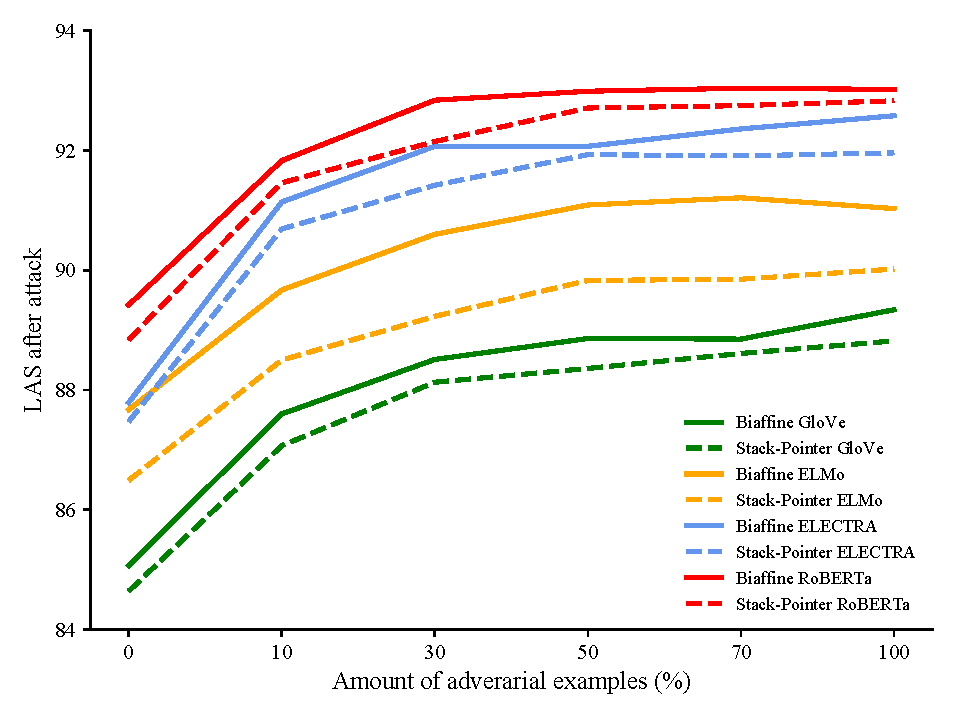
\includegraphics[width=0.7\textwidth]{figures/adv_training_after_attack.pdf}
	\bicaption[fig:ptb-adv-training]{}{PTB-SD-3.3.0上的对抗样本训练实验结果}{Fig.$\!$}{Adversarial trainig results on PTB-SD-3.3.0.}
\end{figure}

具体来说,在PTB-SD-3.3.0上,本文分别测试了在原始训练集数据中增加10\%、30\%、50\%、70\%和100\%的训练集对抗样本后重新训练的分析器的性能和鲁棒性。
训练的分析器包括Biaffine分析器和Stack-Pointer分析器,使用的词向量包括GloVe、ELMo、ELECTRA和RoBERTa。
实验结果如图\ref{fig:ptb-adv-training}所示,其中通过攻击后LAS来反映模型的鲁棒性。
从图中可以发现,所有类别的模型鲁棒性都随着训练中使用的对抗样本数量的增加而增加。
在初始阶段(30\%)之前增长较快,在使用50\%至70\%的对抗样本时鲁棒性增长逐渐趋于平缓。
但不少模型(如使用GloVe词向量的Biaffine模型)在使用100\%的训练集对抗样本时鲁棒性仍然在增长。

为了反映使用对抗样本训练的模型在原始规范测试集上的性能,表\ref{tbl:ptb-adv-train-result}给出了PTB-SD-3.3.0上使用100\%训练集对抗样本的对抗样本训练实验结果。
其中括号里的数值表示该模型与使用相同类别分析器及词向量,但不使用对抗样本训练的分析模型之间的差距。
从表中可以发现,通过对抗样本训练,所有类别的模型的鲁棒性都得到了显著提升。
而经过对抗样本训练的模型在原始规范文本组成的测试集上的性能并没有受到太大影响。
甚至对某些模型来说(例如使用ELMo词向量的Stack-Pointer模型),使用对抗样本训练还能略微提升其在原始测试集上的性能。

\begin{table}[htbp]
	\bicaption[tbl:ptb-adv-train-result]{}{PTB-SD-3.3.0上的对抗样本训练实验结果}{Table$\!$}{Adversarial training results on PTB-SD-3.3.0.}
    \vspace{0.5em}\centering\wuhao
	\begin{tabular}{lccccc}
		\toprule[1.5pt]
		\multirow{2}{*}{词向量}& \multicolumn{2}{c}{原始结果} & \multicolumn{2}{c}{攻击后结果} & \multirow{2}{*}{攻击成功率\%} \\
		\cmidrule(r){2-3} \cmidrule(r){4-5}
		& UAS & LAS & UAS & LAS & \\
		\midrule[1pt]
		\multicolumn{6}{c}{Biaffine} \\
		\hline
		%GloVe &95.36 & 93.49 &88.69 &85.09 &55.3 \\
		GloVe &95.32 (-0.04) & 93.45 (-0.04) &91.90 (+3.21) &89.34 (+4.25) &38.5 (-16.8) \\
		%ELMo &96.29 &94.51  &90.70 &87.67 &47.5 \\
		ELMo &96.17 (-0.12) &94.37 (-0.14) &93.49 (+2.79) &91.03 (+3.36) &33.2 (-14.3) \\
		%ELECTRA &97.12 & 95.38 &91.05 &87.79 &50.6 \\
		ELECTRA &96.96 (-0.16) & 95.23 (-0.15) &95.03 (+3.98) &92.58 (+4.79) &33.4 (-17.2) \\
		%RoBERTa &97.09 & 95.41 &92.14 &89.42 &46.1 \\
		RoBERTa &97.03 (-0.06) & 95.30 (-0.11) &95.30 (+3.16) &93.02 (+3.60) &29.5 (-16.6) \\
		\hline
		\multicolumn{6}{c}{Stack-Pointer} \\
		\hline
		%GloVe &94.93 & 93.05 &88.26 &84.64 &52.6 \\
		GloVe &94.92 (-0.01) & 93.04 (-0.01) &91.58 (+3.32) &88.82 (+4.18) &36.2 (-16.4) \\
		%ELMo &95.69 & 93.77 &89.57 &86.49 &46.8 \\
		ELMo &95.75 (+0.06) & 93.81 (+0.04) &92.64 (+3.07) &90.02 (+3.53) &34.1 (-12.7) \\
		%ELECTRA &96.94 & 95.19 &90.69 &87.47 &50.3 \\
		ELECTRA &96.83 (-0.11) & 95.04 (-0.15) &94.53 (+3.84) &91.96 (+4.49) &34.2 (-16.1) \\
		%RoBERTa &96.93 & 95.20 &91.58 &88.84 &45.1 \\
		RoBERTa &96.80 (-0.13) & 95.01 (-0.19) &95.10 (+3.52) &92.83 (+3.99) &29.1 (-16.0) \\
		\bottomrule[1.5pt]
	\end{tabular}
\end{table}

\iffalse
\begin{table}[htbp]
	\bicaption[tbl:adv-train-result]{}{对抗样本训练实验结果}{Table$\!$}{Adversarial training results.}
    \vspace{0.5em}\centering\wuhao
	\begin{tabular}{lccccc}
		\toprule[1.5pt]
		\multirow{2}{*}{词向量}& \multicolumn{2}{c}{原始结果} & \multicolumn{2}{c}{攻击后结果} & \multirow{2}{*}{攻击成功率\%} \\
		\cmidrule(r){2-3} \cmidrule(r){4-5}
		& UAS & LAS & UAS & LAS & \\
		\midrule[1pt]
		\multicolumn{6}{c}{Biaffine} \\
		\hline
		GloVe &95.36 & 93.49 &88.69 &85.09 &55.3 \\
		GloVe* &95.32 & 93.45 &91.90 &89.34 &38.5 \\
		\hline
		ELMo &96.29 &94.51  &90.70 &87.67 &47.5 \\
		ELMo* &96.17 &94.37  &93.49 &91.03 &33.2 \\
		\hline
		ELECTRA &97.12 & 95.38 &91.05 &87.79 &50.6 \\
		ELECTRA* &96.96 & 95.23 &95.03 &92.58 &33.4 \\
		\hline
		RoBERTa &97.09 & 95.41 &92.14 &89.42 &46.1 \\
		RoBERTa* &97.03 & 95.30 &95.30 &93.02 &29.5 \\
		\hline
		\multicolumn{6}{c}{Stack-Pointer} \\
		\hline
		GloVe &94.93 & 93.05 &88.26 &84.64 &52.6 \\
		GloVe* &94.92 & 93.04 &91.58 &88.82 &36.2 \\
		\hline
		ELMo &95.69 & 93.77 &89.57 &86.49 &46.8 \\
		ELMo* &95.75 & 93.81 &92.64 &90.02 &34.1 \\
		\hline
		ELECTRA &96.94 & 95.19 &90.69 &87.47 &50.3 \\
		ELECTRA* &96.83 & 95.04 &94.53 &91.96 &34.2 \\
		\hline
		RoBERTa &96.93 & 95.20 &91.58 &88.84 &45.1 \\
		RoBERTa* &96.80 & 95.01 &95.10 &92.83 &29.1 \\
		\bottomrule[1.5pt]
	\end{tabular}
\end{table}
\fi



\subsection{基于模型融合的鲁棒性增强方法}[Robustness Increasing Approach Based on Model Ensemble]
\label{sec:chapter3-ensemble}

在第\ref{sec:chapter3-results}节的分析实验中,本章证明了针对不同分析模型生成的对抗样本都是不同的。
基于此发现,本章提出使用模型融合方法提升依存分析模型的鲁棒性。
在前文中探讨了跨随机种子、跨模型和跨词向量三种对抗样本迁移情况。
由于不同的依存分析模型之间差异巨大,难以实现模型融合,本节仅对跨随机种子模型融合和跨词向量模型融合方法进行实验。

具体来说,假设有A和B两个模型需要融合,对于基于图的Biaffine分析模型,本章首先分别用模型A和模型B对输入句子进行分析,获取每两个词之间存在弧的分数,然后将模型A和模型B得到的分数相加,用于解码过程生成目标依存结构。
对于基于转移的IT-BS和Stack-Pointer分析模型,本章在每个转移状态下分别使用模型A和模型B对下一个要执行的转移动作进行预测,获取每个转移动作的分数,然后将模型A和模型B得到的分数相加,选择分数之和最高的转移动作作为接下来要执行的动作。

\begin{figure}[hbtp]
	\centering
	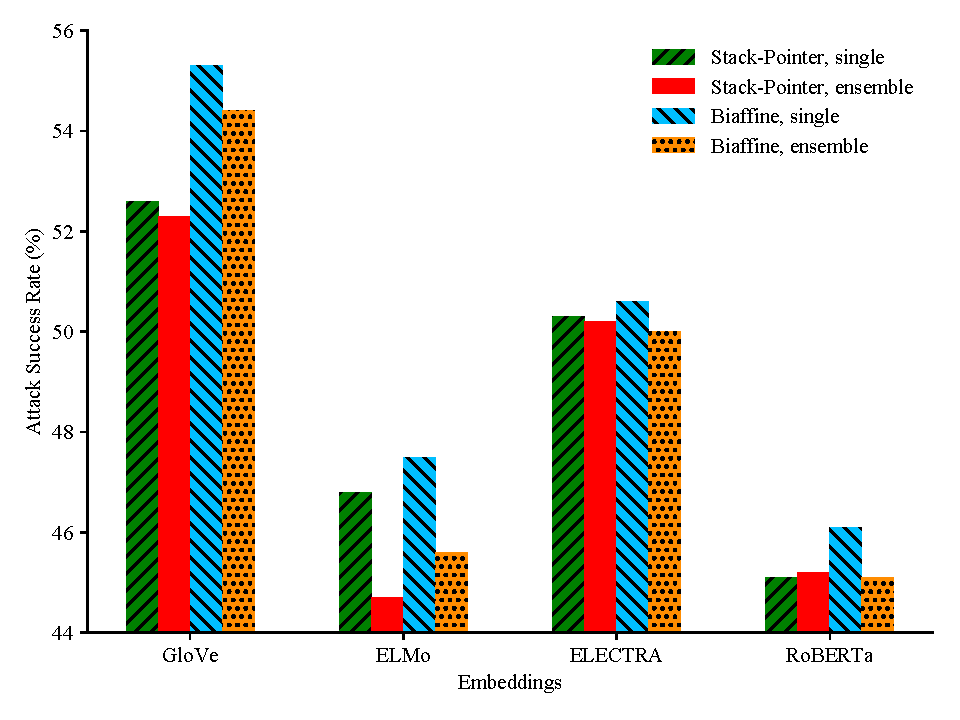
\includegraphics[width=0.7\textwidth]{figures/ensemble_seed_attack_succ.pdf}
	\bicaption[fig:ptb-cross-seed-ensemble]{}{PTB-SD-3.3.0上的跨随机种子模型融合实验结果}{Fig.$\!$}{Cross-seed ensemble results on PTB-SD-3.3.0.}
\end{figure}

图\ref{fig:ptb-cross-seed-ensemble}给出了在PTB-SD-3.3.0上使用Biaffine分析器和Stack-Pointer分析器分别进行跨随机种子模型融合的实验结果,以攻击成功率呈现。
实验结果表明,对于绝大部分分析模型,跨随机种子模型融合都能有效降低攻击成功率,增强其鲁棒性。
只有使用RoBERTa作为输入的Stack-Pointer模型的在进行跨随机种子模型融合鲁棒性没有增强。
另外,在图中所示的四种词向量中,模型融合方法对于使用ELMo的分析模型鲁棒性增强效果最好。

\begin{table}[htbp]
	\bicaption[tbl:ptb-cross-embed-ensemble]{}{PTB-SD-3.3.0上的跨词向量模型融合实验结果}{Table$\!$}{Cross-embedding ensemble results on PTB-SD-3.3.0.}
    \vspace{0.5em}\centering\wuhao
	\begin{tabular}{lccccc}
		\toprule[1.5pt]
		\multirow{2}{*}{词向量}& \multicolumn{2}{c}{原始结果} & \multicolumn{2}{c}{攻击后结果} & \multirow{2}{*}{攻击成功率\%} \\
		\cmidrule(r){2-3} \cmidrule(r){4-5}
		& UAS & LAS & UAS & LAS & \\
		\midrule[1pt]
		\multicolumn{6}{c}{Biaffine} \\
		\hline
		RoBERTa        &97.09 & 95.41 &92.14 &89.42 &46.1 \\
		+GloVe     &97.16 & 95.55 &92.39 &89.77 &43.8 \\
		+ELMo   &97.20 & 95.58 &92.53 &89.97 &42.5 \\
		+ELECTRA &\bf97.25 &\bf95.63 &\bf92.73 &\bf90.12 &\bf41.5 \\
		\hline
		\multicolumn{6}{c}{Stack-Pointer} \\
		\hline
		RoBERTa        &96.93 & 95.20 &91.58 &88.84 &45.1 \\
		+GloVe     &97.01 & 95.32 &92.15 &89.49 &43.4 \\
		+ELMo   &96.98 & 95.26 &\bf 92.28 &89.62 &42.3 \\
		+ELECTRA &\bf 97.14 &\bf 95.45 &92.27 &\bf 89.64 &\bf 41.5 \\
		\bottomrule[1.5pt]
	\end{tabular}
\end{table}

表\ref{tbl:ptb-cross-embed-ensemble}给出了在PTB-SD-3.3.0上使用Biaffine分析器和Stack-Pointer分析器分别进行跨词向量模型融合的实验结果。
为了更清晰地展现该方法的有效性,表中将使用鲁棒性最强的RoBERTa词向量训练的分析模型作为基础,并逐步将使用另外三种词向量训练的分析模型与其融合。
从实验结果中可以发现,每一种新的词向量训练的模型的加入都使融合模型的鲁棒性得到了增强。
而同时融合四种词向量训练的分析模型得到的融合模型同时在原始结果和攻击后结果上取得了最好性能,针对此模型的攻击成功率也是最低的。

值得注意的是,相比于第\ref{sec:chapter3-adv-training}节中使用的对抗样本训练方法,本节提出的模型融合方法不仅在原始测试数据集上不会带来性能下降,反而会有一定提升。
除此之外,对抗样本训练方法需要提前获取对抗样本,而且有使得模型过拟合到对抗样本的风险。
而模型融合方法在训练时只需要使用原始训练集,且没有过拟合到对抗样本的风险。
但相对的,模型融合方法需要多个分析模型同时预测,在使用时会占用更多的计算资源。

\section{本章小结}[Conclusions]

本章针对语义依存图分析模型性能在非规范文本上显著下降的问题,首先设计了针对基于神经网络的依存分析模型的对抗样本攻击算法。
该算法使用多种方法生成并过滤候选词,保证候选词的数量和质量,从而生成流畅性和依存结构不变性有保障的对抗样本。
本章接着利用该攻击算法对现有各种类型的依存分析模型和作为模型输入的词向量的鲁棒性进行深入探索,并发现:
(1)测试样本中的未登录词和训练集中未出现过的词是导致依存分析模型误判的重要原因;
(2)攻击算法针对不同类别分析器、不同词向量甚至不同初始化随机种子训练的分析模型生成的对抗样本都不同。
基于这两点发现,本章提出了对抗样本训练和模型融合方法,有效增强了现存的基于神经网络的依存分析模型的鲁棒性。

% Local Variables:
% TeX-master: "../thesis"
% TeX-engine: xetex
% End: